\documentclass[preprint,12pt,authoryear]{elsarticle}
\usepackage[T1]{fontenc}
\usepackage[utf8]{inputenc}
\usepackage{amsmath,amssymb}
\usepackage{booktabs}
\usepackage{array}
\usepackage{longtable}
\usepackage{graphicx}
\usepackage{microtype}
\usepackage{multirow}
\usepackage[section]{placeins}
\usepackage{pgfplots}
\pgfplotsset{compat=1.17}
\usepackage[hidelinks]{hyperref}
\usepackage{lineno}
\biboptions{round,authoryear}

% \journal{Decision Support Systems}  % restore when actually submitting
\makeatletter
\def\ps@pprintTitle{\let\@oddhead\@empty\let\@evenhead\@empty
  \def\@oddfoot{\footnotesize\itshape Manuscript in preparation\hfill\today}\let\@evenfoot\@oddfoot}
\makeatother

\newcommand{\dE}{\Delta E}
\newcommand{\pp}{\,pp}

\begin{document}

\begin{frontmatter}

\title{Operational autonomy of LLM-based decision support under provider withdrawal: shared errors, diversity caps and model families}

\author{Andrew V. Strizhevskiy (strizhevskiyav@student.bmstu.ru)}
\author{Egor D. Verkhovykh (verkhovyykhed@student.bmstu.ru)}
\author{Daniil M. Paramonov (paramonovdm@student.bmstu.ru)}
\author{Maxim I. Kolosov (kolosovm@bmstu.ru)}
\address{Bauman Moscow State Technical University, Moscow, Russia}

\begin{abstract}
Decision-support systems can combine several large language models (LLMs), and access to them can be lost in groups: all models of one developer, or all models offered only through an API. We propose a withdrawal stress test that treats an LLM portfolio as a system of components and measures its operational autonomy with reliability importance measures: the error increase under group withdrawal, its ratio form (risk achievement worth) and joint importance. Hypotheses and decision rules were fixed in an internal, hash-recorded protocol and validated on synthetic panels before real answers were analysed. Using item-level answers of 70 models to 14,038 MMLU questions, a replication on MMLU-Pro, 13 local runs and pair data on 349 leaderboard models, we find that losing any single developer costs at most 0.6 percentage points of error, whereas restricting a system to open-weight models costs 2.3--2.9 points on MMLU and about 5.2 on MMLU-Pro. Models of one developer share wrong answers beyond item difficulty, robustly on MMLU and weakly on MMLU-Pro. None of three tested selection methods beat a cap of one model per developer, and an independence-based assessment overstates the withdrawal cost about fivefold. Fine-tuned models keep much of their base model's error pattern. At 8--12 billion parameters no accuracy deficit of Russian models was detected on MMLU, which does not establish equivalence. The results support withdrawal testing and a per-developer cap; counting model families rather than brands remains a design hypothesis, because a direct test showed no conclusive advantage of a family cap over the developer cap.
\end{abstract}

\begin{keyword}
decision support systems \sep large language models \sep model ensembles \sep correlated errors \sep reliability importance measures \sep technology sovereignty
\end{keyword}

\end{frontmatter}


\section{Introduction}

Decision-support systems (DSS) are adopting large language models (LLMs) as components that answer questions, classify documents and draft recommendations. In the energy sector they are proposed as copilots for power-system operations \citep{sulaima2026trustworthy}, as dispatch agents \citep{zhao2026dispatch} and for operational reliability evaluation \citep{cheng2026reliability}, typically with a single model kept in an advisory role. A robust design rarely relies on a single model: answers of several models are aggregated by a vote or a learned combiner, or requests are routed among models \citep{jiang2023blender,wang2025moa,chen2024frugalgpt,ong2025routellm}. This design has a dependency that average-accuracy evaluations ignore. The models come from a small number of developers, and access to them can be lost in groups. A developer can deprecate a model family, change its terms or stop serving a jurisdiction; all models available only through a hosted API can become unavailable at once, a form of the vendor lock-in long discussed for cloud services \citep{oparamartins2016}. For organisations in critical sectors, the choice of models is therefore also a question of technology sovereignty, defined in the innovation-policy literature as the ability of a state to provide the technologies it deems critical, developing them or sourcing them from other economic areas without one-sided structural dependency \citep{edler2023}. For some operators it is also a compliance question: in Russia, companies in the energy and fuel sectors are among the subjects of the critical information infrastructure \citep{fz187}, and since 1 January 2025 government bodies and regulated customers may not use foreign software on its significant objects \citep{ukaz166}.

We study the component reliability of such systems: each LLM is a component whose answers may be wrong, and the system's reliability is the accuracy of the aggregated answer. This paper asks three questions that a DSS designer faces. (i) How much accuracy does an aggregated system retain when a group of models is withdrawn? (ii) How should the models and the aggregation rule be chosen to limit that loss? (iii) What does a new, for example domestic, model add, and does a fine-tune of a foreign base model behave as an independent component? We answer them with a \emph{withdrawal stress test} that treats an LLM portfolio as a system of components and uses the importance measures that reliability engineering developed for components that fail together \citep{birnbaum1969,vesely1983,borgonovo2001,honglie1993}. In the terms of power-system planning, the test is an N$-$1 check of the portfolio (any single developer is lost), extended to pairs of developers (N$-$2) and to the common-cause loss of all API-only models.

Three features shape the study. First, the null model controls item difficulty and the popularity of each wrong option, so that shared errors are not confused with shared hard questions \citep{eckhardt1985}. Second, hypotheses, decision rules and analysis settings were fixed in a written, hash-recorded internal protocol and validated on synthetic panels with known ground truth before any real answer was analysed; later amendments and post-hoc analyses are listed with their timing (\ref{app:amend}). Third, the analysis uses public evaluation records and our released local runs, so the results can be reproduced without access to hosted models.

Our contributions are:
\begin{enumerate}
\item A withdrawal stress test for LLM portfolios that maps group-withdrawal loss, its ratio form and joint importance onto the importance measures of probabilistic safety assessment, with synthetic validation of the tests and of the coverage of their intervals.
\item A like-for-like cost of restricting a system to open-weight models on two benchmarks, and a comparison with independence- and difficulty-based predictions of the withdrawal cost.
\item Evidence, replicated more weakly on a second benchmark (where the developer-jackknife interval includes zero), that developer-level shared errors survive a difficulty-calibrated test under several agreement measures once accuracy is matched, and that none of the three tested selection methods beat a one-model-per-developer cap: on MMLU its held-out worst case (11.65\%) equals that of accuracy-greedy selection (11.65\%) and is slightly better than that of robustness-oriented selection (11.81\%); a gain of the cap appears only on MMLU-Pro (11.10\% vs 13.10\%; approximate intervals).
\item A quantification of error inheritance from base to fine-tuned models, primarily at item level with a difficulty null for six related local pairs, supported by a pair-level analysis of public leaderboard models in which a direct fine-tuning link adds shared errors beyond the architecture-and-size class of a model family.
\end{enumerate}

\section{Related work}

\paragraph{Combining LLMs} LLM outputs are combined by ranking and fusion \citep{jiang2023blender}, by layered architectures in which models refine each other's answers \citep{wang2025moa}, by cascades that query cheaper models first \citep{chen2024frugalgpt} and by learned routers \citep{ong2025routellm}. These methods optimise quality and cost when all models are available. LLMs also enter DSS research directly, for example to turn model explanations into narratives \citep{martens2025}. The robustness of such combinations to the loss of their components has, to our knowledge, not been studied.

\paragraph{Correlated errors of LLMs} \citet{kim2025correlated} measured agreement on wrong answers for 349 open models on the Open LLM Leaderboard and 71 models on HELM, and found that models from the same company and with the same architecture agree more often when both are wrong. Their measure compares agreement with a constant chance level, and the authors list the lack of a difficulty control as a limitation. \citet{goel2025great} proposed a chance-adjusted, accuracy-conditional agreement measure (CAPA) and showed that similar models favour each other as judges; they exclude same-developer pairs as a confound rather than studying them. Our developer-level test replicates the direction of \citet{kim2025correlated}; its additions are calibration against a simulated world with shared difficulty and wrong-option popularity, a minimal detectable effect, a second benchmark, and a comparison of agreement measures.

\paragraph{Algorithmic monoculture} In a stylised model of firms selecting candidates, relying on one shared, more accurate ranking can lower overall decision quality compared with independent assessments \citep{kleinberg2021monoculture}. Empirically, sharing training data increases the rate at which the same instances are failed by all systems, while sharing a foundation model does not always do so \citep{bommasani2022picking}, and across commercial prediction APIs from different providers, instances failed by all systems are more frequent than independence predicts \citep{toups2023ecosystem}. These works study homogeneous outcomes across decision makers; we study what a single system loses when a correlated group of its models is withdrawn, and we measure dependence against a difficulty-calibrated null rather than against independence.

\paragraph{Lineage of LLMs} Lineage leaves traces in model outputs: phylogenies can be recovered from output similarity \citep{yax2025phylolm}, and ErrorTrace attributes a model to its base family from its error set \citep{zang2025errortrace}. These works use lineage for attribution; they do not report how much of a base model's failure pattern a derivative keeps relative to accuracy-matched unrelated models, nor what this implies for ensembles.

\paragraph{Ensemble diversity and benchmark quality} Diversity is the classical design principle of classifier ensembles \citep{kuncheva2003,brown2005}; its measures are computed on a fixed team and mix every source of coincident failure. \citet{turkmen2026} select LLM ensembles greedily by mutual information under correlated errors, for full availability. Benchmark labels are imperfect: a re-annotation found errors in about 6.5\% of MMLU questions \citep{gema2025mmlu}, which matters for agreement measures because strong models share ``wrong'' answers on mislabelled items. Leaderboard rankings move under small changes of option order, answer symbols and scoring method \citep{alzahrani2024benchmarks}, accuracy and the rate of unparsable answers change under meaning-preserving changes of prompt format \citep{sclar2024format}, and contamination inflates MMLU scores \citep{zhao2025mmlucf}.

\paragraph{Reliability engineering} Importance measures rank components by their effect on system risk: Birnbaum importance \citep{birnbaum1969}, risk achievement worth (risk with a component failed relative to nominal; \citealp{vesely1983}), the differential importance measure, which, unlike risk achievement worth and Fussell--Vesely importance, is additive over groups \citep{borgonovo2001}, and joint importance, the second-order interaction of two components \citep{honglie1993}. Guidelines for common-cause failure analysis treat a shared manufacturer or design as a coupling factor and diversity as a defence, while cautioning that diverse components sharing parts should not be assumed fully independent \citep{mosleh1998ccf}. Resilience metrics separate the loss after a disruption from the subsequent recovery \citep{henry2012,hosseini2016}. Common-cause failures are multiple failures of components from shared root causes \citep{iaea1992ccf}. In multiversion software, independently developed versions fail independently only if the probability of failure is the same for every input; whenever it varies across inputs, coincident failures exceed the independence prediction \citep{eckhardt1985}, as an experiment confirmed \citep{knight1986}. Developing versions with diverse methodologies lowers the probability of simultaneous failure and can, in theory, even beat independence, but it guarantees no level of reliability in practice \citep{littlewood1989}. We use this vocabulary directly: the null model is the coincident-failure baseline of shared input difficulty, developer and family effects are common-cause dependences beyond it, and the withdrawal measures are importance measures applied to groups of models.

\section{Problem formulation and measures}

\subsection{Setting}
A panel of LLMs answers $N$ multiple-choice items with correct keys $y_k$. Model $i$ gives answer $a_{ik}$. A \emph{portfolio} $P$ is a set of $n$ models combined by an aggregation rule; its error $E(P)$ is the share of items on which the aggregate answer is wrong. A \emph{withdrawal scenario} $W$ removes a group of models: all models of one developer, or all API-only models (models whose weights are not published for local deployment). Under withdrawal the system re-fits its rule on the remaining models. For API-only models, withdrawal means loss of access. For open-weight developers it is a weaker scenario, loss of future versions and support, because published weights can be held locally.

\subsection{Withdrawal measures}
Following the importance measures of probabilistic safety assessment, we report
\begin{align}
\dE_W &= E(P\setminus W) - E(P), \\
\mathrm{RAW}_W &= E(P\setminus W)/E(P), \\
\mathrm{JI}(W_1,W_2) &= E(P\setminus(W_1\cup W_2)) - E(P\setminus W_1) - E(P\setminus W_2) + E(P).
\end{align}
$\dE_W$ is the primary measure and corresponds to the loss term of resilience metrics \citep{henry2012}; recovery by replacement is not modelled. In the classification of \citet{hosseini2016}, the withdrawal measures are therefore static, performance-based measures of a system's absorptive capacity. $\dE_W$ and $\mathrm{RAW}_W$ are the interval and ratio forms of risk achievement worth, the increase in risk when a feature is removed or assumed failed \citep{vesely1983}. $\mathrm{JI}$ is a finite-difference analogue, on error, of joint reliability importance \citep{honglie1993}: positive when losing two groups together costs more than the two losses added. With withdrawal as failure and error as one minus reliability, JI equals minus their joint reliability importance, so a positive JI means that the two groups substitute for each other. It is needed because RAW-type measures are not additive over groups \citep{borgonovo2001}. Because $\dE$ of a given portfolio depends on how that portfolio was selected, we also report a like-for-like \emph{sovereignty cost} $C = E(P_{\text{open}}) - E(P_{\text{cap}})$, the error of the best five-model open-weight portfolio minus the error of the diversity-cap portfolio under full availability, with paired bootstrap intervals, and its variant $C'$, in which the five-model open-weight portfolio is replaced by the best open-weight option, a single model or a vote, whichever errs less.

\subsection{Null models}
N1 (independence): each model is correct with its own probability and wrong answers are uniform over distractors. N2 (conditional independence given the item): correctness follows a one-parameter item-response model with guessing, $P(\text{correct}) = g + (1-g)\,\sigma(\theta_i - b_k)$ with $g$ one over the number of options, and wrong answers are drawn from the item's pooled distribution of wrong answers $w_k$. N2 keeps item difficulty and the popularity of each wrong option and removes every other dependence; it was chosen over a two-parameter model in the synthetic validation by a pre-stated rule.

\subsection{Hypotheses}
\textbf{H1 (developer-level shared errors).} Let $S_{ij}$ be the number of items on which models $i$ and $j$ give the same wrong answer, with N2 expectation $E_{ij} = \sum_k (1-p_{ik})(1-p_{jk}) \sum_o w_{ko}^2$, and excess $x_{ij} = (S_{ij}-E_{ij})/N$. The statistic $T$ is the mean over developers of the mean within-developer excess, minus the mean excess of between-developer pairs matched to each within pair on both accuracies (within 0.03, widened up to 0.12 until five pairs match) and on exact prompt text. H1 is supported if the one-sided parametric-bootstrap $p$-value under N2 is below 0.05 and $T$ exceeds the minimal detectable effect established in simulation; refuted if the developer-jackknife 90\% interval lies below that effect.

\textbf{H2 (the most accurate rule is not the most robust).} For portfolios of the $n \in \{3,5,7,9\}$ most accurate models, the rule with the lowest full-availability error differs from the rule with the lowest worst-case error over withdrawal scenarios, by at least 1 point in both, for at least two sizes. Refuted if at every size the full-availability winner is also, or within 0.5 points of, the worst-case winner.

\textbf{H3 (robust selection beats a diversity cap).} Scenario-robust selection minimises $(1-\lambda)E(P) + \lambda \max_W E(P\setminus W)$ with $\lambda = 0.5$; a scenario that empties a portfolio counts as error 0.75 (guessing). Evaluated leave-one-developer-out, it must lower the held-out worst-case error relative to a cap of at most one model per developer by at least 1 point. Refuted if the cap is as good or better within 0.5 points.

The aggregation rules are the best single model, plurality vote (ties broken by the summed accuracy of each option's voters), a log-odds weighted vote, Dawid--Skene \citep{dawidskene1979} and stacking. Comparators for H3 are accuracy-greedy selection, the diversity cap and a plug-in mutual-information heuristic in the spirit of, but not identical to, the estimator of \citet{turkmen2026}.

\section{Data and procedure}

\subsection{Benchmarks and panels}
The Holistic Evaluation of Language Models project \citep{liang2023helm} publishes the answer of every evaluated model to every item. The primary data are HELM's MMLU \citep{hendrycks2021mmlu} runs: 14,038 four-option items in 57 subjects, 5-shot prompts, temperature 0. After deduplication of snapshots and aliases by a rule written from model names before outcomes were examined, the panel has 70 models from 18 developers, 42 open-weight and 28 API-only (Table~\ref{tab:data}). Prompts differ only in an optional leading format instruction; exact prompt text is a matching variable in H1, and the 30 models with the modal prompt on every item form a sensitivity panel. The replication uses HELM's MMLU-Pro runs \citep{wang2024mmlupro}: 1,000 items with up to ten options and chain-of-thought answers sampled at temperature 1. Answers were parsed from the reasoning text; eight of 66 models whose parsed correctness agreed with HELM's own scoring on fewer than 95\% of items were excluded from the primary panel by a pre-stated rule, leaving 58 models from 15 developers, 31 of them API-only.

We also ran 12 open models locally on the exact HELM MMLU prompts, with greedy decoding, at most eight output tokens and quantised weights (mostly 4-bit Q4\_K\_M; GigaChat3.1 6-bit and GigaChat-20B 5-bit, as published by their developers): eight Russian models (YandexGPT-5-Lite-8B, T-lite-it-2.1, GigaChat3.1-10B-A1.8B, GigaChat-20B-A3B, Vikhr-Nemo-12B, saiga\_\allowbreak nemo\_\allowbreak 12b, saiga\_\allowbreak yandexgpt\_\allowbreak 8b, Cotype-Nano) and four foreign anchors (Qwen2.5-7B, Qwen3-8B, Llama-3.1-8B, Mistral-Nemo-12B). Two Russian models declare a foreign base (T-lite-it-2.1: Qwen3-8B; Vikhr-Nemo: Mistral-Nemo), and two are fine-tunes of a base named in the model name (saiga\_nemo: Mistral-Nemo; saiga\_yandexgpt: YandexGPT-5-Lite). A thirteenth, larger Russian model, T-pro-it-2.1 (32B, a fine-tune of Qwen3-32B), was run later on all items (post hoc). For population-scale inheritance we use the public pair table of \citet{kim2025correlated}, with MMLU-Pro agreement statistics for all pairs of 349 Open LLM Leaderboard models, joined with the leaderboard's self-declared base-model field; 60,031 pairs have metadata for both models.

\begin{table}[!htbp]
\centering
\caption{Data sources.}
\label{tab:data}
\small
\resizebox{\textwidth}{!}{%
\begin{tabular}{@{}lrrrl@{}}
\toprule
Source & Models & Items & Developers & Answers \\
\midrule
HELM MMLU (primary) & 70 & 14,038 & 18 & item level, temperature 0 \\
HELM MMLU-Pro (replication) & 58 & 1,000 & 15 & item level, chain of thought, temperature 1 \\
Local runs (this study) & 12 & 14,038 & 9 & item level, greedy, quantised \\
Open LLM Leaderboard \citep{kim2025correlated} & 349 & -- & -- & MMLU-Pro pair statistics only \\
\bottomrule
\end{tabular}}
\end{table}

\subsection{Estimation}
Items are split into two cross-fitting folds (by subject on MMLU, at random on MMLU-Pro); selection and fitting use one fold and evaluation the other, and estimates combine both directions. Intervals come from a cluster bootstrap over subjects on MMLU and over items on MMLU-Pro (200 resamples), with every selection and fit repeated inside each resample; joint importance uses a bootstrap interval centred on the estimate and inflated by $\sqrt{G/(G-1)}$. H1 uses 200 N2 parametric-bootstrap panels (100 in sensitivity panels) and a developer jackknife. The primary portfolio has $n=5$ models selected by accuracy-greedy plurality. Analysis code was written in Python (with AI assistance, see Acknowledgements); its correctness was checked on synthetic panels with known ground truth and by reproducing every reported statistic from stored outputs.

\subsection{Synthetic validation before real data}
Before any real answer was analysed, the tests were run on 600 synthetic panels generated with developer and lineage factors, item difficulty, wrong-option preferences and 3\% wrong keys, on a provisional 64-model structure close to the real panel. The first version of H1, based on withdrawal losses of single developers, had correct size but power of at most 0.12, because removing a few models from a 64-model vote barely changes it. H1 was therefore replaced by the pairwise statistic above. A further check showed that an unmatched comparison was biased under the null, because models of one developer have similar abilities and similar-ability models share answers on mislabelled items; this led to accuracy matching. The final H1 has size 0.050, power 1.00 from a factor standard deviation of 0.2, and a minimal detectable effect of $T=0.0028$. Nominal 95\% intervals had validated coverage of 0.91 for $\dE$ and 0.94 for JI; JI point estimates showed a slight upward bias (16 of 22 misses below the interval). The admission chart recovered true gains within 0.1 points. For MMLU-Pro a first size check failed (0.070); a re-check adopted after that failure (new seeds for size, fixed subject shifts for coverage) passed size (0.050), but $\dE$ coverage reached 0.896, so MMLU-Pro intervals were approximate and decisions there rest on the H1 test and point estimates. Because the percentile intervals under-covered, every $\dE$ interval reported below is calibrated on these synthetic panels (post hoc): both half-widths around the point estimate are multiplied by the factor $k$ that gives 95\% coverage, chosen on a random half of the panels and checked on the other half, over 200 splits. This gives $k = 1.12$ on MMLU (5--95\% range over splits 1.04--1.30; median out-of-sample coverage 0.951) and $k = 1.17$ on MMLU-Pro (1.05--1.30; 0.949). The calibration is validated for $\dE$ only; for the sovereignty costs $C$ and $C'$, which compare two portfolios, the same factor is applied as an approximation, so their nominal 95\% level is not validated. All these intervals reflect item sampling only; model sampling is assessed separately with a leave-one-developer-out jackknife (\ref{sec:supp}).

\section{Results}

\subsection{Developer-level shared errors (H1)}
By the pre-specified decision rule H1 is supported on both benchmarks, firmly on MMLU and weakly on MMLU-Pro (Table~\ref{tab:hyp}). On MMLU, two models of one developer give the same wrong answer on 0.46 percentage points more items (about 65 of 14,038) than accuracy- and prompt-matched pairs of different developers ($T = 0.00462$, $p \le 0.005$, where 0.005 is the smallest value attainable with 200 null panels; 90\% jackknife interval $[0.00162, 0.00762]$), about 13 null standard deviations from the N2 mean in the pre-specified run and 1.65 times the minimal detectable effect. The result holds in all four sensitivity panels: strict prompt ($T=0.00991$), without the largest developer (0.00422), without models below 40\% accuracy (0.00458) and open-weight models only (0.00595). On MMLU-Pro, $T=0.00414$ ($p \le 0.005$) exceeds its minimal detectable effect of 0.00358, but the support is weaker: the jackknife interval includes zero in the primary panel and in three of five sensitivity panels, the panel without models below 40\% accuracy is inconclusive ($T=0.00304$), and in a post-hoc diagnostic, without the pair of models of one developer (Writer) the statistic falls to $T=0.00151$, below the minimal detectable effect of 0.00358.

The developer effect also holds under the agreement measures of \citet{kim2025correlated} and CAPA \citep{goel2025great} once accuracy is matched, and without the MMLU items flagged as erroneous by MMLU-Redux (\ref{sec:supp}).

\begin{table}[!htbp]
\centering
\caption{Pre-specified hypotheses: decisions on both benchmarks.}
\label{tab:hyp}
\small
\begin{tabular}{@{}p{3.4cm}p{4.6cm}p{4.6cm}@{}}
\toprule
Hypothesis & MMLU (70 models) & MMLU-Pro (58 models) \\
\midrule
H1 developer-level shared errors & supported; $T=0.0046$, $p\le0.005$; robust in 4 sensitivity panels & supported; $T=0.0041$, $p\le0.005$; jackknife interval includes 0; one panel inconclusive; below the minimal detectable effect without Writer \\
H2 accuracy--robustness trade-off of rules & refuted; voting rules within 0.5\pp & inconclusive; single frontier model best but fragile, below threshold \\
H3 robust selection beats the cap & refuted; gain $-0.16$\pp\ $[-0.63, 0.20]$ & refuted; gain $-2.00$\pp\ (approximate interval $[-4.61, -0.30]$) \\
\bottomrule
\end{tabular}
\end{table}



\subsection{Aggregation rules and selection (H2, H3)}
On MMLU the four voting rules (plurality, weighted vote, Dawid--Skene, stacking) differ by at most 0.5 points under full availability and in the worst case, at every portfolio size, and the best single model is more than one point worse; H2 is refuted. On MMLU-Pro a single frontier model (Gemini 3 Pro preview, error 9.80\%) is the most accurate rule at $n=3$ and 5, but under withdrawal of its developer it falls to 14.00\% while the voting rules keep 12.30--13.90\%. The direction is the one H2 predicted, but the full-availability gaps (0.5 and 0.9 points) miss the 1-point threshold: inconclusive.

H3 is refuted on both benchmarks (Table~\ref{tab:h3}): none of the three tested selection methods (accuracy-greedy, scenario-robust with $\lambda = 0.5$, mutual information) beat the one-model-per-developer cap. This concerns these methods and settings only; it does not show that no robustness optimiser, ensemble size or scenario set could do better. On MMLU the cap has the lowest full-availability error (10.91\%), and its held-out worst case (11.65\%) equals that of accuracy-greedy selection (11.65\%) and is slightly better than that of scenario-robust selection (11.81\%). A gain of the cap appears only on MMLU-Pro, where its held-out worst case is 11.10\% against 13.10\% for scenario-robust selection (approximate intervals). The held-out evaluation covers single-developer withdrawals; the API-only scenario is always part of the training family. The plug-in mutual-information heuristic is worst on both benchmarks; on MMLU-Pro it collapses (57.2\%) once its strongest developer is withdrawn, because it selects weak models whose answers look informative. This concerns our heuristic, not the estimator of \citet{turkmen2026}. The MMLU refutations of H2 and H3 hold in all three sensitivity panels.

\begin{table}[!htbp]
\centering
\caption{Portfolio selection ($n=5$, plurality): error in \%, full availability and held-out worst case under leave-one-developer-out withdrawal. MMLU-Pro values have approximate intervals.}
\label{tab:h3}
\small
\begin{tabular}{@{}lrrrr@{}}
\toprule
& \multicolumn{2}{c}{MMLU} & \multicolumn{2}{c}{MMLU-Pro} \\
\cmidrule(lr){2-3}\cmidrule(lr){4-5}
Selection & Full & Worst case & Full & Worst case \\
\midrule
Diversity cap ($\le$1 per developer) & 10.91 & 11.65 & 9.80 & 11.10 \\
Accuracy-greedy & 11.06 & 11.65 & 10.90 & 14.80 \\
Scenario-robust ($\lambda=0.5$) & 11.12 & 11.81 & 10.70 & 13.10 \\
Plug-in mutual information & 11.75 & 12.65 & 13.60 & 57.20 \\
\bottomrule
\end{tabular}
\end{table}

\subsection{Cost of withdrawal}
The primary MMLU portfolio (Claude 3.5 Sonnet, Yi 34B, Gemini 1.5 Pro, DeepSeek-V3, GPT-4o) errs on 11.06\% [8.89, 14.65] of items. Withdrawing all API-only models raises its error to 13.24\% ($\dE = 2.19$ [1.13, 5.64], RAW 1.20 [1.11, 1.60]); the remaining vote reduces, through the tie-break, to the best single open-weight model, DeepSeek-V3. Single developers cost less: Anthropic 0.59 [0.22, 1.35], DeepSeek 0.46 [$-0.03$, 0.87], Google 0.38 [0.02, 0.99], OpenAI 0.27 [$-0.14$, 0.74]; in power-system terms, the worst single-developer (N$-$1) loss is 0.59 points. Withdrawals interact: for every pair of Anthropic, DeepSeek, Google and OpenAI, losing both costs more than the two losses added (JI from 0.60 [0.21, 1.00] to 1.26 [0.57, 1.91]; JI point estimates may be slightly biased upwards), consistent with a vote that degrades faster as it shrinks.

The like-for-like sovereignty cost $C$ is 2.86 points [1.78, 3.47] on MMLU (cap 10.91\% against the five-model open-weight vote, 13.77\%). On MMLU, however, the best open-weight option is a single open model, DeepSeek-V3 (13.24\%), which is better than the open-weight five-model vote; against it the cost is $C' = 2.33$ points [1.36, 3.03]. Restricting the system to open-weight models therefore costs 2.3--2.9 points on MMLU. On MMLU-Pro both forms give 5.20 points [2.51, 8.36] (9.80\% against 15.00\%), because there the best open option is the ensemble of open models (15.00\%), which beats the best single open model (16.30\%). In a post-hoc leave-one-developer-out jackknife, $C$ stays positive whichever developer is removed; a heuristic range that adds this model-sampling uncertainty to the item-sampling interval gives [0.22, 5.35] on MMLU and [0.10, 10.56] on MMLU-Pro. This range is not a confidence interval with a validated level; it only shows that the sign of $C$ survives both sources of variation (\ref{sec:supp}). The autonomy margin rests on a single strong open model: without DeepSeek's models in the panel, withdrawing the API-only models would cost 7.62 points. Figure~\ref{fig:chain} summarises the MMLU error under availability restrictions. On the 936 engineering-science items, pre-specified as a proxy for technical questions in the energy sector, the primary portfolio errs more often (15.81\%), and withdrawing API-only models changes its error by 0.43 points (to 16.24\%, about four questions; no interval computed), too few questions to compare with the 2.19 points on all of MMLU; an unweighted vote of all models loses about 2 points (24.89\% to 26.92\%); a compute-constrained open portfolio of models with at most 100 billion parameters errs on 19.03\% of all items.

\begin{figure}[!htbp]
\centering
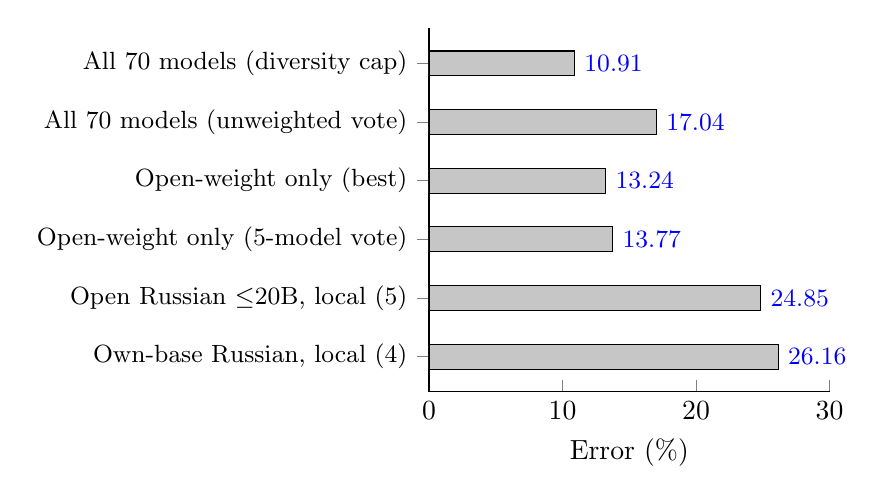
\begin{tikzpicture}
\begin{axis}[
  xbar, width=0.55\textwidth, height=6.2cm, xmin=0, xmax=30,
  xlabel={Error (\%)}, ytick={1,2,3,4,5,6},
  yticklabels={{Own-base Russian, local (4)}, {Open Russian $\le$20B, local (5)}, {Open-weight only (5-model vote)}, {Open-weight only (best)}, {All 70 models (unweighted vote)}, {All 70 models (diversity cap)}},
  y tick label style={font=\small}, nodes near coords, nodes near coords style={font=\small},
  bar width=9pt, enlarge y limits=0.12, axis x line*=bottom, axis y line*=left]
\addplot+[xbar, fill=gray!45, draw=black] coordinates {
  (10.91,6) (17.04,5) (13.24,4) (13.77,3) (24.85,2) (26.16,1)};
\end{axis}
\end{tikzpicture}
\caption{Error on HELM MMLU by available model set. ``Open-weight only (best)'' is the primary portfolio after withdrawal of API-only models, which reduces to DeepSeek-V3. Russian-model portfolios use the 12 local runs; ``Russian models (5)'' includes two fine-tunes of foreign bases, and ``own-base'' excludes them (post hoc). An unweighted vote of all 70 models is worse than a well-chosen portfolio.}
\label{fig:chain}
\end{figure}

\paragraph{Independence-based assessment overstates the cost} Re-running the primary pipeline on 100 panels simulated under each null model shows how an assessment that ignores dependence would err (MMLU, descriptive; Table~\ref{tab:null}). Under independence (N1), a five-model vote would err on about 1\% of items and API-only withdrawal would cost 10.2 points, about five times the observed 2.19; no N1 panel came as low as the observation. N2 comes close on the withdrawal cost (2.59 [2.00, 2.91]; 12\% of panels at or below the observed value) but predicts a more accurate ensemble than observed in all 100 panels (10.00\% against 11.06\%). Real errors are more dependent than item difficulty implies, so the members of a vote contribute less than a difficulty-only model suggests.

\begin{table}[!htbp]
\centering
\caption{Observed portfolio error and API-only withdrawal cost against null-model predictions (MMLU; 100 simulated panels each; mean [5th, 95th percentile]; descriptive).}
\label{tab:null}
\small
\resizebox{\textwidth}{!}{%
\begin{tabular}{@{}lrr@{}}
\toprule
& Portfolio error (\%) & $\dE$, API-only withdrawn (pp) \\
\midrule
N1, independence & 1.22 [1.05, 1.38] & 10.23 [4.42, 17.37] \\
N2, item difficulty and wrong-option popularity & 10.00 [9.64, 10.37] & 2.59 [2.00, 2.91] \\
Observed & 11.06 & 2.19 \\
\bottomrule
\end{tabular}}
\end{table}

\paragraph{Admission of new models} A model-based admission chart, fitted to the 42 open-weight models, evaluates a sixth model added to the open-weight portfolio (error 13.77\%) on a grid of accuracies $\{0.50, 0.70, 0.85\}$ and copying rates $\{0, 0.3, 0.6\}$. Only the accuracy of 0.85, about that of the strongest members, gives a gain: 0.96 points with errors independent of the panel given the item and 0.40 points when the candidate copies the panel's answer 60\% of the time; all candidates at 0.50 and 0.70 make the vote worse. Because real errors are more dependent than the chart's generator allows, its zero-copying column is likely optimistic.

\subsection{Domestic models}
The best Russian model, YandexGPT-5-Lite-8B, answers 73.3\% of MMLU items correctly; the best open model in the HELM panel, DeepSeek-V3, answers 86.8\% (Table~\ref{tab:local}). For the foreign anchors also evaluated by HELM, local and hosted answers agree on 91\% (Qwen2.5-7B) and 87\% (Mistral-Nemo) of items, with accuracy within 0.4 points; Llama-3.1-8B agrees on 75\% and is 8.7 points less accurate locally, of which at most 3.8 points come from answers that are a sentence rather than a letter. Unrelated local pairs are no more similar than local--HELM pairs of similar accuracy (mean excess 0.0096 against 0.0138), so local deployment does not make models look alike. Quantisation changes individual answers but not accuracy: an 8-bit run of Qwen2.5-7B is as accurate as the 4-bit run (71.6\% vs 71.3\%; hosted 71.4\%) but agrees with the hosted run on 97.4\% of items instead of 91.1\% (post hoc). Three local runs were redone after their first accuracies were seen, because their packaged chat templates were missing or broken: saiga\_yandexgpt (0.290 to 0.663 after restoring its official template), YandexGPT-5-Lite (0.729 to 0.733) and 61 over-long GigaChat3.1 prompts re-run with a larger context. Llama's packaged template is its official one, so its format failures were left as model behaviour.

\begin{table}[!htbp]
\centering
\caption{Local runs on HELM MMLU (14,038 items).}
\label{tab:local}
\small
\resizebox{\textwidth}{!}{%
\begin{tabular}{@{}llrr@{}}
\toprule
Model & Developer (declared base) & Accuracy & Invalid \\
\midrule
YandexGPT-5-Lite-8B & Yandex & 0.733 & 0.0001 \\
T-lite-it-2.1 & T-Bank (Qwen3-8B) & 0.724 & 0.0001 \\
GigaChat3.1-10B-A1.8B & Sber & 0.718 & 0.0002 \\
saiga\_yandexgpt\_8b & I.~Gusev (YandexGPT-5-Lite, by name) & 0.663 & 0 \\
Vikhr-Nemo-12B & Vikhr (Mistral-Nemo) & 0.654 & 0.0019 \\
saiga\_nemo\_12b & I.~Gusev (Mistral-Nemo, by name) & 0.639 & 0.0001 \\
GigaChat-20B-A3B & Sber & 0.616 & 0.0001 \\
Cotype-Nano & MTS AI & 0.539 & 0.0003 \\
\midrule
Qwen2.5-7B & Alibaba & 0.713 & 0.0027 \\
Qwen3-8B (no reasoning) & Alibaba & 0.673 & 0 \\
Mistral-Nemo-12B & Mistral AI & 0.642 & 0 \\
Llama-3.1-8B & Meta & 0.456 & 0.0380 \\
\bottomrule
\end{tabular}}
\end{table}

Adding any Russian model to the open-weight portfolio raises its error by 0.08 to 0.31 points, and greedy re-selection with the Russian models in the pool picks none of them. A portfolio of open Russian models of up to 20B, run locally, errs on 24.85\% [19.69, 32.00], 11.1 points above the open-weight portfolio. In post-hoc size-matched comparisons, the three Russian 8--12B models on Russian bases (YandexGPT-5-Lite, saiga\_yandexgpt, GigaChat3.1) are 2.84 points [1.95, 3.74] more accurate than the foreign 7--12B anchors excluding Llama, and the difference stays positive when any single model is left out (range 1.15 to 4.91); with all six Russian 8--12B models the difference is 1.24 points [0.56, 1.97], but leaving one model out can reverse it. Adding a model of either origin changes the open-weight portfolio by the same amount (difference $-0.01$ [$-0.08$, 0.10]). The intervals resample subjects, not models. Three of the four foreign anchors are 2024 releases, whereas the three Russian own-base models in the comparison are newer, so origin and vintage are confounded; Qwen3-8B was run with reasoning disabled. At 8--12 billion parameters, no accuracy deficit of the Russian models was therefore detected; this is not evidence of equivalence, since the models are a small sample, their release dates differ and the intervals resample subjects, not models; and the gap of the local domestic portfolio is consistent with the scale of the models that could be run. A larger model is consistent with this but does not demonstrate it (post hoc): on all 14,038 MMLU items, T-pro-it-2.1 (32B, a fine-tune of Qwen3-32B by a Russian developer) answers 82.0\% correctly, third among 15 models (14 HELM open models of 27--72B plus T-pro); it is outscored only by Qwen2.5-72B (83.3\%) and Qwen2-72B (82.7\%; mean of the 14: 75.2\%). A first run on a stratified 2,850-item subset (50 per subject) gave 84.1\%, second of 15. By our own rule, however, T-pro belongs to the Qwen family, and it is the only data point above 20B; own-family Russian models in our runs reach at most 73.3\% (YandexGPT-5-Lite-8B), and GigaChat-20B-A3B (about 3B active parameters, going by its name) 61.6\%. Larger open Russian models exist, GigaChat3.1-702B-A36B and GigaChat3.5-432B-A28B \citep{aisage2026gigachat}, but they need hundreds of gigabytes of memory to run locally and were not tested; running them would test the scale hypothesis directly. That the gap reflects scale rather than origin is therefore a hypothesis consistent with the data, not a demonstrated conclusion. T-pro is also newer than most of the HELM models it is compared with, so scale and vintage are confounded. Adding it to the open-weight portfolio as a sixth member changes the error by $-0.26$ points [$-0.56$, 0.26], and greedy re-selection with T-pro in the pool does not pick it, as the admission chart predicts for a candidate below about 85\% accuracy. On a Russian-language test (ruMMLU from the MERA benchmark \citep{fenogenova2024mera}, public test; post hoc), we used two prompts, zero-shot and with five worked examples per domain, and scored both on the same 9,748 items (the worked examples excluded). A cross-fitted plurality vote of three Russian models errs 3.6 points less than one of three foreign models zero-shot and 5.4 points less with worked examples ($-5.42$ [$-6.93$, $-3.48$]); this result is robust. On valid answers only, the three Russian-base models are more accurate than the three foreign anchors under both prompts (+4.71 points zero-shot, +2.12 [+1.14, +3.50] few-shot). For all six Russian 8--12B models the advantage on valid answers depends on the prompt (+2.15 [+1.29, +2.97] zero-shot, $-0.53$ [$-1.43$, +0.62] few-shot), so we do not claim it. With format failures counted as errors, the six Russian 8--12B models are less accurate than the foreign anchors by 2.07 points [1.00, 3.08] zero-shot and 5.25 [2.67, 7.72] few-shot (1.49 and 2.87 under the parser variant), which is what a DSS receiving generated answers would experience; the plurality trio is selected from six Russian against three foreign models. Worked examples do not remove answer-format failures \citep{sclar2024format}: for some models the invalid share rises, because the model re-answers the examples (Vikhr-Nemo 0.22 to 0.38, Llama-3.1-8B 0.08 to 0.45, Qwen3-8B 0.09 to 0.20), and for GigaChat3.1 it stays high (0.40 to 0.36). A post-hoc parser variant that also accepts a Latin letter followed by the option text lowers T-lite's few-shot invalid share from 0.157 to 0.032 and leaves these conclusions unchanged. If foreign base families are withdrawn as well, the Russian models on Russian bases (YandexGPT, saiga\_yandexgpt and both GigaChat models) err on 26.16\%, and voting barely improves on the best single model, because only two independent developers remain.

\subsection{Inheritance of errors}
\paragraph{Item level, local runs} The six related local pairs are three Russian fine-tunes with their foreign bases (Vikhr-Nemo and saiga\_nemo with Mistral-Nemo, T-lite-it-2.1 with Qwen3-8B), one pair of fine-tunes of the same foreign base (Vikhr-Nemo, saiga\_nemo), one Russian fine-tune with its Russian base (saiga\_yandexgpt, YandexGPT-5-Lite) and two models of one developer (GigaChat3.1, GigaChat-20B). For each pair we computed $x_{ij}$ minus its mean over unrelated local pairs matched on both accuracies, with significance from an N2 null (200 panels). All six pairs exceed their comparison pairs ($p\le0.005$, the floor of the test; Figure~\ref{fig:inherit}a). Vikhr-Nemo has a raw excess $x$ of 0.086 with its base, against 0.14--0.16 for the same model run in two deployments (local and HELM), so it keeps roughly half of the agreement of an identical model. The two fine-tunes of Mistral-Nemo share an excess of 0.063 with each other. T-lite-it-2.1, trained further and five points more accurate than its base, keeps less of Qwen3-8B (0.018).

\paragraph{Population scale, Open LLM Leaderboard} This analysis was specified in the internal protocol before any outcome was computed, after the pair counts and the published coefficients of \citet{kim2025correlated} were known. Pairs of leaderboard models are classed as parent--child (one model's declared base is the other; 32 pairs, 8 base families), siblings (same declared base; 737 pairs, 15 families), same architecture class with different declared base (18,132 pairs) and unrelated (41,130 pairs). The statistic is $P(\text{same answer} \mid \text{both wrong})$ minus its mean over unrelated pairs matched on both accuracies within $\pm0.02$, with cluster-bootstrap intervals over base families. Parent--child pairs exceed matched unrelated pairs by 0.167 [0.114, 0.192] and siblings by 0.101 [0.061, 0.288], in every sensitivity analysis. The pre-specified ordering parent--child $>$ siblings $>$ same architecture is not supported; among pairs of equal size, same-architecture pairs (0.246) even exceed parent--child pairs (0.155).

Post-hoc checks show that this depends on how lineage is labelled (Figure~\ref{fig:inherit}b; details in \ref{sec:supp}). With lineage from each model's own card (213 of 349 models; 168 direct parent--child pairs in 64 families), a direct fine-tuning link exceeds a placebo of same-architecture, same-size pairs with different declared bases by 0.101 [0.061, 0.162] for fine-tunes alone, whereas the leaderboard's derived base field shows no such excess.

\begin{figure}[!htbp]
\centering
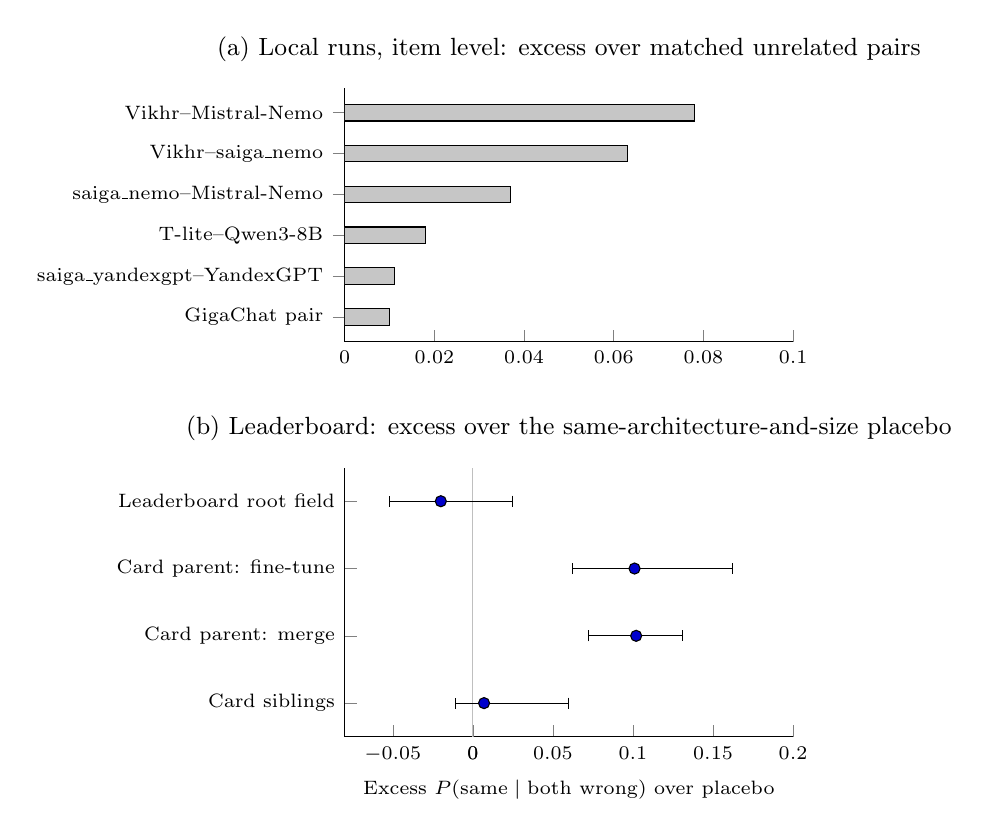
\begin{tikzpicture}
\begin{axis}[name=a, title={(a) Local runs, item level: excess over matched unrelated pairs}, title style={font=\small},
  xbar, width=0.6\textwidth, height=4.8cm, xmin=0, xmax=0.1,
  ytick={1,2,3,4,5,6}, yticklabels={GigaChat pair, saiga\_yandexgpt--YandexGPT, T-lite--Qwen3-8B, saiga\_nemo--Mistral-Nemo, Vikhr--saiga\_nemo, Vikhr--Mistral-Nemo}, enlarge y limits=0.12,
  y tick label style={font=\scriptsize}, x tick label style={font=\scriptsize, /pgf/number format/fixed},
  bar width=6pt, axis x line*=bottom, axis y line*=left, scaled x ticks=false]
\addplot+[xbar, fill=gray!45, draw=black] coordinates {
 (0.010,1) (0.011,2) (0.018,3) (0.037,4) (0.063,5) (0.078,6)};
\end{axis}
\begin{axis}[at={(a.south west)}, anchor=north west, yshift=-1.6cm, title={(b) Leaderboard: excess over the same-architecture-and-size placebo}, title style={font=\small},
  width=0.6\textwidth, height=5cm, xmin=-0.08, xmax=0.2, ymin=0.5, ymax=4.5,
  ytick={1,2,3,4}, yticklabels={Card siblings,Card parent: merge,Card parent: fine-tune,Leaderboard root field}, y tick label style={font=\scriptsize},
  x tick label style={font=\scriptsize, /pgf/number format/fixed}, xlabel={Excess $P(\text{same}\mid\text{both wrong})$ over placebo}, xlabel style={font=\scriptsize},
  axis x line*=bottom, axis y line*=left, extra x ticks={0}, extra x tick style={grid=major}]
\addplot+[only marks, mark=*, black, error bars/.cd, x dir=both, x explicit] coordinates {
 (0.007,1) += (0.053,0) -= (0.018,0)
 (0.102,2) += (0.029,0) -= (0.030,0)
 (0.101,3) += (0.061,0) -= (0.039,0)
 (-0.020,4) += (0.045,0) -= (0.032,0)};
\end{axis}
\end{tikzpicture}
\caption{Error inheritance. (a) Excess same-wrong-answer agreement $x_{ij}$ of related local pairs over unrelated local pairs matched on accuracy (all $p\le0.005$ against an N2 null). (b) Post hoc: excess conditional agreement of related pairs over a placebo of same-architecture, same-size pairs with a different declared base, with 95\% family-bootstrap intervals; ``leaderboard root field'' uses the leaderboard's derived base field, the other rows use base models declared in model cards. The scales of (a) and (b) differ.}
\label{fig:inherit}
\end{figure}

\section{Discussion}

\subsection{Implications for DSS design}
The results support five design rules for LLM-based decision support that must keep working when providers are lost. \emph{First, test withdrawal scenarios, not only average accuracy, and repeat the test when the portfolio changes.} Group-withdrawal loss is measurable with standard importance measures, and positive joint importance shows that losses compound as a portfolio shrinks. \emph{Second, do not assess withdrawal risk under independence.} An independence-based assessment overstated the API-only withdrawal cost about fivefold; a model that keeps item difficulty came close on the cost but overstated how much the ensemble's members contribute. \emph{Third, a cap of one model per developer is a simple and effective diversity rule.} Neither the choice among voting rules nor scenario-robust selection improved on it on either benchmark, and it is transparent and cheap; combined with the fourth rule, it would become a cap per model family. \emph{Fourth, count model families rather than brands.} This rule is a design hypothesis. In a post-hoc test (\ref{sec:supp}), a family-based cap selected the same portfolios as the developer cap in the 70-model panel, where the most accurate models already come from distinct developers and families. In the 12 local runs, where fine-tunes share families, it replaced saiga\_yandexgpt with Vikhr-Nemo, raising full-availability error by 0.49 points [0.00, 0.82] and lowering the worst single-family withdrawal by 0.32 [$-0.39$, 0.25]. The direct test therefore shows no conclusive advantage: the family rule trades some accuracy for protection against losing a family. We recommend counting families when assessing a portfolio's diversity, but not yet as a validated selection rule. Fine-tunes keep much of their parent's error pattern beyond what their model family shares, and fine-tunes of one pretrained base resemble each other; a portfolio that counts them as independent suppliers overstates its diversity. This concerns redundancy, not availability: the weights of a fine-tune remain usable when its base's developer stops serving, but the fine-tune gives only partial independent protection against that family's errors. \emph{Fifth, admit a new model only if it is about as accurate as the strongest members.} No Russian or foreign model of up to 20B improved the open-weight portfolio, nor did the 32B T-pro-it-2.1 as a sixth member; a model's contribution follows its accuracy, not its origin.

\subsection{Implications for technology sovereignty}
Restricting the system to open-weight models costs 2.3--2.9 points of error on MMLU and about 5.2 on the harder MMLU-Pro. For a system that answers 1,000 operator queries of comparable difficulty, this means about 23--29 additional wrong answers on MMLU and 52 on MMLU-Pro, against roughly 109 and 98 wrong answers with all models available. On MMLU the best open configuration is a single strong open model, on MMLU-Pro a small open ensemble; without DeepSeek's models the MMLU withdrawal cost would rise from 2.19 to 7.62 points, so autonomy depends on access to at least one strong open-weight family. Within the conditions of this study (English multiple-choice questions, models up to 20 billion parameters run locally), no accuracy deficit of the Russian models was detected at matched size, although origin and vintage are confounded there, and they are neither better nor worse portfolio members than foreign models of that size. The 11-point gap of a portfolio of small, locally run domestic models is consistent with a gap in the scale of locally runnable models, but this remains a hypothesis: the only data point above 20B, T-pro-it-2.1 (32B, a fine-tune of Qwen3-32B by a Russian developer), is outscored by only two of the 14 HELM open models of 27--72B, yet by our rule it belongs to the Qwen family, and own-family Russian models in our runs reach at most 73.3\%. If the hypothesis holds, operational autonomy depends on the capacity to run large open-weight models, such as the open 432B and 702B GigaChat models, and on the diversity of model families more than on the nationality of the developer. The admission chart quantifies the bar for a new model: it must be about as accurate as the strongest open models, and its errors must not copy theirs.

\subsection{Relation to reliability engineering}
Coincident failure on hard inputs \citep{eckhardt1985,knight1986} corresponds to our N2 null: in the Eckhardt--Lee model, independent development yields independent failures only if difficulty does not vary across inputs \citep{littlewood2001review}. Item response models have been fitted to MMLU correctness data of many LLMs \citep{maiapolo2024tiny}; N2 uses a simpler one-parameter model with a guessing floor. Developer and family effects are common-cause dependences beyond N2 \citep{iaea1992ccf}; the gap between N2 predictions and observed withdrawal costs is their effect at the system level. A per-developer cap is a simple form of forced diversity, which in multiversion software lowers coincident failure without guaranteeing reliability \citep{littlewood1989}; here none of the tested selection methods beat the cap. Conventional ensemble diversity measures \citep{kuncheva2003} do not separate these sources of coincidence and do not address the loss of members; the withdrawal measures do.

\subsection{Threats to validity}
\emph{Construct validity.} Multiple-choice accuracy on general benchmarks is a proxy for the reliability of an LLM component in a DSS; it ignores decision costs, task context and users. The engineering-science subset is only a proxy for sector-specific questions, and on it the API-only withdrawal changed the error by only 0.43 points (about four of 936 questions; no interval computed), too few to compare with all of MMLU, so whether the headline cost transfers to technical questions is open. Russian-language performance was measured only for the local models, post hoc, with a zero-shot and a five-example prompt; under both, answer-format failures confound accuracy, and the advantage of all six Russian models on valid answers depends on the prompt; MERA itself scores ruMMLU by log-likelihood, whereas we parse generated answers, as a DSS would receive them, so our accuracies are not comparable with MERA leaderboard values. A single fixed prompt per benchmark is used, and prompt format can change accuracy substantially \citep{sclar2024format}. \emph{Internal validity.} About 6.5\% of MMLU items are mislabelled \citep{gema2025mmlu}; excluding the items flagged by that re-annotation changed none of the conclusions, but unflagged label noise may remain. ``Developer'' bundles shared data, training, post-training and serving. Models differ in their preferences for answer letters, even within a family \citep{alzahrani2024benchmarks}; a post-hoc null in which each model draws its wrong answers with its own letter preferences leaves the developer effect unchanged ($T=0.00466$, $p\le0.005$), so shared letter bias does not explain it. Conversely, part of what N2 attributes to item difficulty may itself be shared model properties \citep{toups2023ecosystem}, which would make the H1 test conservative. Contamination of MMLU \citep{zhao2025mmlucf} may raise accuracies but is not expected to create developer-specific agreement beyond shared training data, which the developer effect already includes. The size-matched, own-base, measure-comparison and leaderboard-robustness analyses are post hoc, and in the size-matched comparison the Russian models are newer than most foreign anchors; three local runs were corrected after their first accuracies were seen, by restoring official chat formats; the superseded runs are kept. \emph{Statistical conclusion validity.} H1 on MMLU-Pro leans on one developer pair; percentile intervals under-covered (0.91 for $\dE$ on MMLU, 0.896 on MMLU-Pro) and were calibrated on synthetic panels, which assumes that the synthetic generator represents the real sampling variability; the null-model comparison is descriptive; the leaderboard analysis uses pair-level statistics and self-declared lineage (model-card base models for 213 of 349 models), and its results depend on how lineage is labelled; group comparisons of local models resample subjects, not models; a developer jackknife shows that model sampling dominates the uncertainty of the withdrawal measures. \emph{External validity.} Local runs are quantised; 4-bit weight quantisation usually changes accuracy little but can change individual answers \citep{li2024quant}, and our 8-bit check showed unchanged accuracy with higher answer agreement with the hosted model; the largest Russian model we ran has 32B parameters, whereas open Russian models of 432B and 702B parameters exist; hosted domestic models were not evaluated; and model panels change quickly.

\section{Conclusion}
A withdrawal stress test built on reliability importance measures makes the operational autonomy of LLM-based decision support measurable. On two benchmarks, restricting a system to open-weight models costs 2.3--2.9 points of error on MMLU and 5.2 on MMLU-Pro; none of the three tested selection methods beat a one-model-per-developer cap, whose held-out worst case on MMLU equals that of accuracy-greedy selection (11.65\%) and which gains only on MMLU-Pro (11.10\% vs 13.10\%); and independence-based assessment overstates the stakes. Developer-level shared errors are clear on MMLU but weak on MMLU-Pro, where the developer-jackknife interval includes zero and the statistic without the Writer pair (0.00151) is below the minimal detectable effect (0.00358). Whether the weaker local domestic portfolio reflects model scale rather than origin remains a hypothesis consistent with the data. Fine-tuned models keep much of their parent's failure pattern, at item level and across hundreds of public models, beyond what their model family shares. The next steps are sector-specific tasks with decision costs, non-English questions, item-level population data and runs of the largest open domestic models.

\section*{Data and code availability}
All analysis scripts, the protocol with its amendment history and hashes, all stored outputs and the local model answers (including superseded runs) are available at https://github.com/AndrewStrizhevskiy/withdrawal-stress-test. HELM raw results are public, and the repository contains the scripts that download and parse them. The Open LLM Leaderboard pair table is available from the repository of \citet{kim2025correlated} and is not redistributed.

\section*{Acknowledgements}
The authors are grateful to Anthropic for the Claude AI assistant, which supported the preparation of the analysis code and the editing of the manuscript.

\section*{Declaration of generative AI and AI-assisted technologies in the writing process}
During the preparation of this work the authors used Claude (Anthropic) to assist with analysis code and with editing the text. The authors directed the study, reviewed and verified the analyses and the text, and take full responsibility for the content of the publication.

\section*{Declaration of competing interest}
The authors declare no competing interests.

\appendix
\section{Protocol amendments, post-hoc analyses and pre-specified outputs}
\label{app:amend}
\footnotesize
The protocol is internal: it was hash-recorded before each stage but not registered externally with an independent timestamp. Some decisions were changed after the synthetic checks (amendments A2--A5), three local runs were corrected after their first accuracies were seen, and several analyses were specified only after other results were known; all are listed below with their timing and marked post hoc in the text. Not every result therefore stems from the original, unchanged plan.

{\renewcommand{\arraystretch}{1.25}%
\begin{longtable}{@{}>{\raggedright\arraybackslash}p{0.13\textwidth}>{\raggedright\arraybackslash}p{0.52\textwidth}>{\raggedright\arraybackslash}p{0.31\textwidth}@{}}
\toprule
Change & Content & Timing relative to data \\
\midrule
\endhead
A1 & Concrete synthetic-validation settings and pass criteria & before validation; no data \\
A2 & H1 statistic replaced by pairwise excess same-wrong agreement; difficulty-recovery criterion replaced by replicate reliability & after the first synthetic run failed; no real data \\
A2.1 & Accuracy matching of comparison pairs in H1 & during implementation; no real data \\
A3 & Targeted re-validation of joint-importance intervals & no real data \\
A4 & Prompts differing only in a leading format instruction treated as equivalent; prompt as matching variable; strict panel as sensitivity & after seeing which models the strict rule excludes; before any answer was analysed \\
Exact prompts & H1 matching on exact prompt text (documented after the run started; implemented before) & before any statistic was seen \\
A5 & MMLU-Pro validation re-check adopted after a failed size check (0.070): new seeds for size, fixed subject shifts for coverage; fallback to approximate intervals & no real outcomes \\
Local runs & Official chat formats restored for three models; one context-window re-run & after first accuracies (post hoc) \\
Local designs & Bridge, inheritance and admission analyses of local runs & specified before the local runs; after the MMLU results \\
Leaderboard & Inheritance at scale & specified before outcomes; after counts and published coefficients were known \\
Post hoc & Size-matched and own-base comparisons; measure comparison; sovereignty cost $C$; leaderboard placebo, depth and triplets; model-card lineage; developer jackknife & specified before computing; after earlier results \\
MMLU-Redux & Pre-specified exclusion sensitivity, run late & specified before the data; run after the main results \\
Not run & S1b-type outputs on MMLU-Pro & -- \\
\bottomrule
\end{longtable}}


\section{Supplementary results}
\label{sec:supp}
\normalsize
This appendix collects post-hoc robustness analyses summarised in the main text. Each was specified in the internal protocol before it was computed.

\paragraph{Alternative agreement measures} The conclusion does not depend on the agreement measure (post hoc, Table~\ref{tab:measures}). With the same accuracy and prompt matching, the conditional agreement of \citet{kim2025correlated} and CAPA \citep{goel2025great} give developer contrasts 9.6 to 16.8 null standard deviations above their N2 values. Without accuracy matching, the raw same-wrong-answer rate is fully explained by shared difficulty and ability (observed contrast 0.0062 against 0.0059 under N2). The essential control is therefore conditioning on accuracy; the N2 simulation adds calibration of every measure against the same difficulty-only world.

\begin{table}[!htbp]
\centering
\caption{H1 developer contrast under alternative agreement measures (MMLU, 70 models; post hoc). Observed contrast, its mean under a separate set of 200 N2 panels, and $z = $ (observed $-$ N2 mean)/N2 standard deviation.}
\label{tab:measures}
\small
\resizebox{\textwidth}{!}{%
\begin{tabular}{@{}lrrrrrr@{}}
\toprule
& \multicolumn{3}{c}{Accuracy- and prompt-matched} & \multicolumn{3}{c}{Unmatched} \\
\cmidrule(lr){2-4}\cmidrule(lr){5-7}
Measure & Observed & N2 mean & $z$ & Observed & N2 mean & $z$ \\
\midrule
Excess over N2, $x_{ij}$ (H1) & 0.00462 & 0.00005 & 14.1 & 0.00036 & 0.00013 & 0.8 \\
Raw same-wrong rate & 0.00581 & 0.00118 & 13.6 & 0.00624 & 0.00587 & 1.2 \\
$P(\text{same}\mid\text{both wrong})$ & 0.01756 & $-0.00034$ & 9.6 & 0.01422 & $-0.00178$ & 9.4 \\
CAPA & 0.01850 & $-0.00026$ & 16.8 & 0.01028 & $-0.00060$ & 10.5 \\
\bottomrule
\end{tabular}}
\end{table}

\paragraph{Exclusion of mislabelled items} On MMLU, the pre-specified exclusion of the 374 items flagged as erroneous by MMLU-Redux \citep{gema2025mmlu} leaves the result unchanged ($T=0.00447$, $p\le0.005$, jackknife interval $[0.00151, 0.00743]$); the same exclusion changes the sovereignty cost $C$ from 2.86 to 2.85 points, $\dE$(API-only) from 2.19 to 2.26 and the H3 gain from $-0.16$ to $-0.12$.

\paragraph{Calibrated intervals} Percentile bootstrap intervals for $\dE$ under-covered on the synthetic panels (0.912 over 454 intervals on MMLU, 0.896 over 431 on MMLU-Pro). Scaling both half-widths by $k$ chosen for 95\% coverage on half of the panels and evaluated on the other half (200 splits) gives $k=1.12$ on MMLU and $k=1.17$ on MMLU-Pro, with median out-of-sample coverage 0.951 and 0.949; with all synthetic dependence levels on MMLU, $k=1.14$. Calibration widens, for example, $\dE$(API-only) from [1.24, 5.28] to [1.13, 5.64] and makes the DeepSeek interval include zero ([$-0.03$, 0.87]). Applying $k$ to $C$ and $C'$ is an approximation, because the validation covers $\dE$. The heuristic range for $C$ that includes model sampling combines, separately for each side, the calibrated item-sampling half-width and $1.96$ times the leave-one-developer-out jackknife standard error (18 developers on MMLU, 15 on MMLU-Pro; standard errors 1.23 and 2.21 points) in quadrature. This assumes that the two sources are independent and that the jackknife error is roughly normal; with few developers and one dominant open model neither assumption is secure, so the range has no validated confidence level.

\paragraph{Family-based cap} Family labels equal developers except that Google splits into PaLM~2, Gemini and Gemma, and Upstage Solar Pro joins Phi (its preview model card states that it scales Phi-3-medium). With five models, a family cap, a developer cap and a joint cap select identical portfolios in both folds of the 70-model panel (full error 10.91\%, worst single-developer and single-family withdrawal 11.65\%), also without the Solar merge and with Gemma merged into Gemini. In the 12 local runs, with the pre-existing lineage labels, the developer cap selects YandexGPT-5-Lite, GigaChat3.1, T-lite, Qwen2.5 and saiga\_yandexgpt; the family cap replaces saiga\_yandexgpt with Vikhr-Nemo. Family minus developer cap (200 subject resamples): full error $+0.49$ [0.00, 0.82], worst single-family withdrawal $-0.32$ [$-0.39$, 0.25], worst single-developer withdrawal $+0.30$ [$-0.17$, 0.53]. This analysis is exploratory.

\paragraph{Developer jackknife} Model sampling matters more than item sampling: in a post-hoc leave-one-developer-out jackknife, $C$ stays positive whichever developer is removed (2.15 to 3.48 on MMLU, 4.10 to 6.80 on MMLU-Pro), whereas $\dE$(API-only) ranges from 1.68 to 7.62 and is largest without DeepSeek, when no strong open model remains. The largest gain of robust selection over the cap in the same jackknife is 0.07 points, so the H3 refutation does not depend on any single developer.

\paragraph{Leaderboard lineage, placebo and triplets} Post-hoc robustness checks show that this conclusion depends on how lineage is labelled (Figure~\ref{fig:inherit}b). Against a placebo of same-architecture, same-size ($\pm$10\%) pairs with different declared bases, the leaderboard's derived base field gives no detectable parent--child excess ($-0.020$ [$-0.052$, 0.025]; 31 pairs, 8 families). That field records a root, often missing or self-referential, which lumps distant descendants together. With lineage taken instead from each model's own card (\texttt{base\_model}, available for 213 of the 349 models), there are 168 direct parent--child pairs in 64 families. They exceed matched unrelated pairs by 0.309 [0.279, 0.341] and the same-architecture, same-size placebo by 0.101 [0.073, 0.134]. Fine-tuning links alone give the same excess over the placebo (0.101 [0.061, 0.162]; 65 pairs, 17 families), as do merges (0.102 [0.072, 0.131]); card siblings do not exceed their placebo (0.007 [$-0.011$, 0.060]). A direct fine-tuning link therefore carries shared errors beyond what the architecture-and-size class explains. Whether two fine-tunes of one parent resemble each other more than the parent depends on the parent: across 123 card-lineage triplets the sibling excess is lower than the mean child--parent excess (family-weighted $-0.021$, 12 families), except where the parent is a pretrained base model (Qwen2.5-14B, Qwen2.5-72B, Qwen2-72B), whose instruction-tuned descendants resemble each other more than the base. This is descriptive, with few families per type. On the Russian-language test, all five fine-tuning pairs among the local runs again share errors beyond the null zero-shot ($p\le0.005$), and four of five with five worked examples (the T-lite--Qwen3-8B pair does not replicate, $-0.014$), whereas the GigaChat pair, related only by developer, does not (zero-shot).

\bibliographystyle{elsarticle-harv}
\bibliography{refs}

\end{document}
